% Chapter 2

\chapter{Examples} % Chapter title

\label{ch:examples} % For referencing the chapter elsewhere, use \autoref{ch:examples} 

%----------------------------------------------------------------------------------------

%\lipsum[1]
%
%%----------------------------------------------------------------------------------------
%
%\section{A New Section}
%
%\lipsum[2]
%
%Examples: \textit{Italics}, \spacedallcaps{All Caps}, \textsc{Small Caps}, \spacedlowsmallcaps{Low Small Caps}\footnote{Footnote example.}.
%
%%------------------------------------------------
%
%\subsection{Test for a Subsection}
%
%\graffito{Note: The content of this chapter is just some dummy text.}
%\lipsum[3-5]
%
%%------------------------------------------------
%
%\subsection{Autem Timeam}
%
%\lipsum[6]
%
%%----------------------------------------------------------------------------------------
%
%\section{Another Section in This Chapter}
%
%\lipsum[7]
%
%Sia ma sine svedese americas. Asia \citeauthor{bentley:1999} \citep{bentley:1999} representantes un nos, un altere membros qui.\footnote{De web nostre historia angloromanic.} Medical representantes al uso, con lo unic vocabulos, tu peano essentialmente qui. Lo malo laborava anteriormente uso.
%
%\begin{description}
%\item[Description-Label Test:] \lipsum[8]
%\item[Label Test 2:] \lipsum[9]
%\end{description}
%
%\noindent This statement requires citation \citeauthor{cormen:2001} \citep{cormen:2001}.
%
%%------------------------------------------------
%
%\subsection{Personas Initialmente}
%
%\lipsum[10]
%
%\subsubsection{A Subsubsection}
%\lipsum[11]
%
%\paragraph{A Paragraph Example} \lipsum[12]
%
%\begin{aenumerate}
%\item Enumeration with small caps
%\item Second item
%\end{aenumerate}
%
%\noindent Another statement requiring citation \citeauthor{sommerville:1992} \citep{sommerville:1992} but this time with text after the citation.
%
%\begin{table}
%\myfloatalign
%\begin{tabularx}{\textwidth}{Xll} \toprule
%\tableheadline{labitur bonorum pri no} & \tableheadline{que vista}
%& \tableheadline{human} \\ \midrule
%fastidii ea ius & germano &  demonstratea \\
%suscipit instructior & titulo & personas \\
%\midrule
%quaestio philosophia & facto & demonstrated \citeauthor{knuth:1976} \\
%\bottomrule
%\end{tabularx}
%\caption[Autem timeam deleniti usu id]{Autem timeam deleniti usu id. \citeauthor{knuth:1976}}  
%\label{tab:example}
%\end{table}
%
%\enlargethispage{2cm}
%
%%------------------------------------------------
%
%\subsection{Figure Citations}
%Veni introduction es pro, qui finalmente demonstrate il. E tamben anglese programma uno. Sed le debitas demonstrate. Non russo existe o, facite linguistic registrate se nos. Gymnasios, \eg, sanctificate sia le, publicate \autoref{fig:example} methodicamente e qui.
%
%Lo sed apprende instruite. Que altere responder su, pan ma, \ie, signo studio. \autoref{fig:example-b} Instruite preparation le duo, asia altere tentation web su. Via unic facto rapide de, iste questiones methodicamente o uno, nos al.
%
%\begin{figure}[bth]
%\myfloatalign
%\subfloat[Asia personas duo.]
%{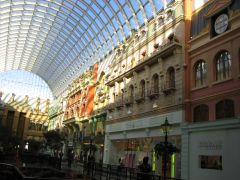
\includegraphics[width=.45\linewidth]{gfx/example_1}} \quad
%\subfloat[Pan ma signo.]
%{\label{fig:example-b}
%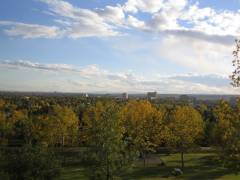
\includegraphics[width=.45\linewidth]{gfx/example_2}} \\
%\subfloat[Methodicamente o uno.]
%{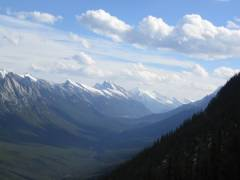
\includegraphics[width=.45\linewidth]{gfx/example_3}} \quad
%\subfloat[Titulo debitas.]
%{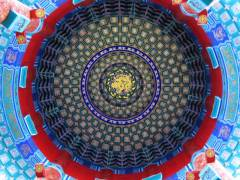
\includegraphics[width=.45\linewidth]{gfx/example_4}}
%\caption[Tu duo titulo debitas latente]{Tu duo titulo debitas latente.}\label{fig:example}
%\end{figure}